\documentclass[12pt]{article}
\usepackage[brazil]{babel}
\usepackage[utf8]{inputenc}
\usepackage[T1]{fontenc}
\usepackage{kpfonts}
\usepackage{graphicx}
\usepackage{geometry}
\usepackage{array}
\usepackage{booktabs}
\usepackage[backend=biber,style=abnt]{biblatex}
\addbibresource{references.bib}
\usepackage[colorlinks=true,linkcolor=black,urlcolor=blue,citecolor=black]{hyperref}
\pagenumbering{gobble} % sem número de página

\begin{document}

% ── CABEÇALHO ──────────────────────────────────────────────────────────────
\noindent
\begin{minipage}[c]{0.5\textwidth}
    \Large\textbf{MC857}\\[0.2em]
    \normalsize Projeto em Sistemas de Informação
\end{minipage}
\hfill
\begin{minipage}[c]{0.2\textwidth}
    \raggedleft
    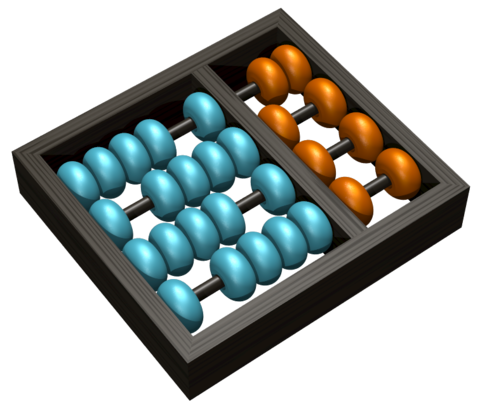
\includegraphics[width=\textwidth]{Logo}
\end{minipage}

\vspace{0.4em}
\noindent\rule{\linewidth}{0.8pt}

% ── TÍTULO ─────────────────────────────────────────────────────────────────
\vspace{1.2em}
\begin{center}
    {\LARGE\textbf{Tema: }\textbf{Simulador de Fórmula 1}}\\[0.6em]
    {\large\textbf{Grupo: }\textit{F1maça}}
\end{center}
\begin{center}
    \begin{tabular}{ll}
        João Guilherme Ferreira Pedra   & RA: 248349 \\
        Luiz Fernando Lima Leite        & RA: 248405 \\
        João Vitor Guilherme dos Santos & RA: 247232 \\
        Caio Zavarezzi Balieiro         & RA: 195260   \\
        Guilherme Resende Braga         & RA: 232517   \\
    \end{tabular}
\end{center}

\vspace{0.8em}
\noindent\rule{\linewidth}{0.8pt}

\vspace{1em}

\section*{Descrição}
O grupo implementará um simulador de corridas de Fórmula 1 baseado em dados reais, em que o usuário configura pilotos, circuitos, pneus e condições climáticas, e acompanha a corrida volta a volta com visualização 2D e momentos-chave em 3D. O backend será desenvolvido em Python com FastAPI e FastF1, comunicando com o frontend React via WebSocket para transmissão dos eventos em tempo real. A visualização 3D será feita com Three.js. Também terá um agente de IA integrado que analisará os eventos da corrida e irá sugerir decisões estratégicas como um engenheiro de pista, usando os dados da simulação como contexto.

\section*{Bases de Dados e Softwares}
FastF1, Ergast API, F1-Tyre-Strategy-Engine Dataset, Ollama, Three.js.

\newpage
\section{Configurações}
Ano especificado: \textbf{2024}
\subsection{Pilotos}
\subsection{Circuitos}
Dados obtidos de \cite{trotman_formula1}.\\
\textbf{Quantidade total de circuitos:} 77.\\
\textbf{Anos dos Dados:} 1982-2026.
\subsubsection{Dados Gerais}circuitos
\begin{enumerate} 
    \item \textbf{Circuits:}
    \begin{itemize} 
        \item \texttt{circuitRef}: identificador textual do circuito; \item \texttt{name}: nome do circuito; 
        \item \texttt{location}: localização do circuito; 
        \item \texttt{country}: país onde está localizado; 
        \item \texttt{lat}: latitude do circuito; 
        \item \texttt{lng}: longitude do circuito; 
        \item \texttt{alt}: altitude do circuito; 
        \item \texttt{url}: endereço da página do circuito. 
    \end{itemize}
    \item \textbf{Constructor Results:}
    \begin{itemize}
        \item \texttt{constructorResultsId}: identificador do resultado;
        \item \texttt{raceId}: identificador da corrida;
        \item \texttt{constructorId}: identificador do construtor;
        \item \texttt{points}: pontos obtidos;
        \item \texttt{status}: situação do resultado.
    \end{itemize}
    
        \item \textbf{Constructor Standings:}
    \begin{itemize}
        \item \texttt{constructorStandingsId}: identificador da classificação;
        \item \texttt{raceId}: identificador da corrida;
        \item \texttt{constructorId}: identificador da equipe;
        \item \texttt{points}: pontos acumulados;
        \item \texttt{position}: posição na classificação;
        \item \texttt{positionText}: posição em formato textual;
        \item \texttt{wins}: número de vitórias.
    \end{itemize}

    \item \textbf{Constructors:}
    \begin{itemize}
        \item \texttt{constructorId}: identificador da equipe;
        \item \texttt{constructorRef}: referência da equipe;
        \item \texttt{name}: nome da equipe;
        \item \texttt{nationality}: nacionalidade da equipe;
        \item \texttt{url}: endereço da página da equipe.
    \end{itemize}

    \item \textbf{Driver Standings:}
    \begin{itemize}
        \item \texttt{driverStandingsId}: identificador da classificação;
        \item \texttt{raceId}: identificador da corrida;
        \item \texttt{driverId}: identificador do piloto;
        \item \texttt{points}: pontos acumulados;
        \item \texttt{position}: posição na classificação;
        \item \texttt{positionText}: posição em formato textual;
        \item \texttt{wins}: número de vitórias.
    \end{itemize}

    \item \textbf{Drivers:}
    \begin{itemize}
        \item \texttt{driverId}: identificador do piloto;
        \item \texttt{driverRef}: referência do piloto;
        \item \texttt{number}: número utilizado pelo piloto;
        \item \texttt{code}: código de três letras do piloto;
        \item \texttt{forename}: primeiro nome;
        \item \texttt{surname}: sobrenome;
        \item \texttt{dob}: data de nascimento;
        \item \texttt{nationality}: nacionalidade do piloto;
        \item \texttt{url}: endereço da página do piloto.
    \end{itemize}

    \item \textbf{Lap Times:}
    \begin{itemize}
        \item \texttt{raceId}: identificador da corrida;
        \item \texttt{driverId}: identificador do piloto;
        \item \texttt{lap}: número da volta;
        \item \texttt{position}: posição ao final da volta;
        \item \texttt{time}: tempo da volta;
        \item \texttt{milliseconds}: tempo da volta em milissegundos.
    \end{itemize}

    \item \textbf{Pit Stops:}
    \begin{itemize}
        \item \texttt{raceId}: identificador da corrida;
        \item \texttt{driverId}: identificador do piloto;
        \item \texttt{stop}: número da parada;
        \item \texttt{lap}: volta em que ocorreu a parada;
        \item \texttt{time}: horário da parada;
        \item \texttt{duration}: duração da parada;
        \item \texttt{milliseconds}: duração em milissegundos.
    \end{itemize}

    \item \textbf{Qualifying:}
    \begin{itemize}
        \item \texttt{qualifyId}: identificador da classificação;
        \item \texttt{raceId}: identificador da corrida;
        \item \texttt{driverId}: identificador do piloto;
        \item \texttt{constructorId}: identificador da equipe;
        \item \texttt{number}: número do carro;
        \item \texttt{position}: posição de largada;
        \item \texttt{q1}: tempo obtido no Q1;
        \item \texttt{q2}: tempo obtido no Q2;
        \item \texttt{q3}: tempo obtido no Q3.
    \end{itemize}

    \item \textbf{Races:}
    \begin{itemize}
        \item \texttt{raceId}: identificador da corrida;
        \item \texttt{year}: ano da temporada;
        \item \texttt{round}: rodada da temporada;
        \item \texttt{circuitId}: identificador do circuito;
        \item \texttt{name}: nome da corrida;
        \item \texttt{date}: data da corrida;
        \item \texttt{time}: horário da corrida;
        \item \texttt{url}: endereço da página da corrida;
        \item \texttt{fp1\_date}: data do primeiro treino livre;
        \item \texttt{fp1\_time}: horário do primeiro treino livre;
        \item \texttt{fp2\_date}: data do segundo treino livre;
        \item \texttt{fp2\_time}: horário do segundo treino livre;
        \item \texttt{fp3\_date}: data do terceiro treino livre;
        \item \texttt{fp3\_time}: horário do terceiro treino livre;
        \item \texttt{quali\_date}: data da classificação;
        \item \texttt{quali\_time}: horário da classificação;
        \item \texttt{sprint\_date}: data da corrida sprint;
        \item \texttt{sprint\_time}: horário da corrida sprint.
    \end{itemize}

    \item \textbf{Results:}
    \begin{itemize}
        \item \texttt{resultId}: identificador do resultado;
        \item \texttt{raceId}: identificador da corrida;
        \item \texttt{driverId}: identificador do piloto;
        \item \texttt{constructorId}: identificador da equipe;
        \item \texttt{number}: número do carro;
        \item \texttt{grid}: posição de largada;
        \item \texttt{position}: posição final;
        \item \texttt{positionText}: posição final em formato textual;
        \item \texttt{positionOrder}: ordem de chegada;
        \item \texttt{points}: pontos obtidos;
        \item \texttt{laps}: voltas completadas;
        \item \texttt{time}: tempo total de corrida;
        \item \texttt{milliseconds}: tempo total em milissegundos;
        \item \texttt{fastestLap}: número da volta mais rápida;
        \item \texttt{rank}: posição da volta mais rápida;
        \item \texttt{fastestLapTime}: tempo da volta mais rápida;
        \item \texttt{fastestLapSpeed}: velocidade da volta mais rápida;
        \item \texttt{statusId}: identificador do status.
    \end{itemize}

    \item \textbf{Seasons:}
    \begin{itemize}
        \item \texttt{year}: ano da temporada;
        \item \texttt{url}: endereço da página da temporada.
    \end{itemize}

    \item \textbf{Sprint Results:}
    \begin{itemize}
        \item \texttt{resultId}: identificador do resultado;
        \item \texttt{raceId}: identificador da corrida;
        \item \texttt{driverId}: identificador do piloto;
        \item \texttt{constructorId}: identificador da equipe;
        \item \texttt{number}: número do carro;
        \item \texttt{grid}: posição de largada;
        \item \texttt{position}: posição final;
        \item \texttt{positionText}: posição final em formato textual;
        \item \texttt{positionOrder}: ordem de chegada;
        \item \texttt{points}: pontos obtidos;
        \item \texttt{laps}: voltas completadas;
        \item \texttt{time}: tempo total da sprint;
        \item \texttt{milliseconds}: tempo total em milissegundos;
        \item \texttt{fastestLap}: número da volta mais rápida;
        \item \texttt{fastestLapTime}: tempo da volta mais rápida;
        \item \texttt{statusId}: identificador do status;
        \item \texttt{rank}: posição da volta mais rápida.
    \end{itemize}

    \item \textbf{Status:}
    \begin{itemize}
        \item \texttt{statusId}: identificador do status;
        \item \texttt{status}: descrição da situação do piloto.
    \end{itemize}

        \item \textbf{Safety Cars:}
    \begin{itemize}
        \item \texttt{Race}: corrida em que o safety car foi utilizado;
        \item \texttt{Cause}: motivo da intervenção;
        \item \texttt{Deployed}: momento em que foi acionado;
        \item \texttt{Retreated}: momento em que foi retirado;
        \item \texttt{FullLaps}: número de voltas completas sob safety car.
    \end{itemize}

    \item \textbf{Fatal Accidents -- Drivers:}
    \begin{itemize}
        \item \texttt{Driver}: piloto envolvido;
        \item \texttt{Age}: idade do piloto no acidente;
        \item \texttt{Date Of Accident}: data do acidente;
        \item \texttt{Event}: evento em que ocorreu o acidente;
        \item \texttt{Car}: carro utilizado;
        \item \texttt{Session}: sessão em que ocorreu o acidente.
    \end{itemize}

    \item \textbf{Fatal Accidents -- Marshals:}
    \begin{itemize}
        \item \texttt{Name}: nome do comissário;
        \item \texttt{Age}: idade no momento do acidente;
        \item \texttt{Date Of Accident}: data do acidente;
        \item \texttt{Event}: evento em que ocorreu o acidente.
    \end{itemize}

    \item \textbf{Red Flags:}
    \begin{itemize}
        \item \texttt{Race}: corrida em que ocorreu a bandeira vermelha;
        \item \texttt{Lap}: volta em que foi acionada;
        \item \texttt{Resumed}: indicação se a corrida foi retomada;
        \item \texttt{Incident}: incidente que causou a interrupção;
        \item \texttt{Excluded}: indicação se o incidente foi desconsiderado.
    \end{itemize}
    
\end{enumerate}





\subsection{Pneus}
Dados obtidos de \cite{tyre_strategy_dataset}. \\
\textbf{Anos dos Dados:} 2023-2024.

\begin{enumerate}
    \item \textbf{Informações completas (final\_merged\_202X\_data):}
        \begin{itemize}
            \item \texttt{Date}: data
            \item \texttt{GP}: nome do Grand Prix
            \item \texttt{RoundNumber}: Rodada (da temporada)
            \item \texttt{Team}: nome do time (Ferrari, Mercedes, etc)
            \item \texttt{Driver}: Abreviação do piloto (HAM, VER, etc)
            \item \texttt{DriverNumber}: identificador do piloto
            \item \texttt{DriverTime}: tempo total do piloto na corrida
            \item \texttt{DriverNumber}: identificador do piloto
            \item \texttt{LapNumber}: volta atual
            \item \texttt{LapTime}: tempo da volta atual
            \item \texttt{Compound}: composto do pneu (HARD, MEDIUM, SOFT, WET, INTERMEDIATE)
            \item \texttt{TyreLife}: número de voltas com o pneu atual na corrida
            \item \texttt{Stint}: Quantidade de períodos contínuos pilotando (da largada ao pitstop, entre pitstops, pitstop até fim da corrida)
            \item \texttt{FreshTyre}: Se o pneu era novo ou não no início do stint (1 para true, 0 para false)
            \item \texttt{DriverNumber}: identificador do piloto
            \item \texttt{Position}: posição atual
            \item \texttt{SessionType}: Free Practice (FP1, FP2, FP3), Qualifying (Q), Race (R)
            \item \texttt{SectorXTime}: tempo do setor (1,2 ou 3) na volta atual
            \item \texttt{SectorXTime}: tempo do setor (1,2 ou 3) na volta atual
        \end{itemize}
\end{enumerate}



\subsection{Condições climáticas}
    \begin{itemize}
        \item \textbf{Time:} O tempo da sessão em que a medição foi feita (útil para sincronizar a mudança de clima com a volta atual do piloto).
        \item \textbf{AirTemp:} Temperatura do ar em graus Celsius ($^\circ$C).
        \item \textbf{TrackTemp:} Temperatura do asfalto em graus Celsius ($^\circ$C) -- crucial para o seu simulador calcular a degradação e a janela de funcionamento do pneu.
        \item \textbf{Humidity:} Umidade relativa do ar (\%).
        \item \textbf{Pressure:} Pressão atmosférica em milibares (mbar).
        \item \textbf{WindSpeed:} Velocidade do vento em metros por segundo (m/s).
        \item \textbf{WindDirection:} Direção do vento em graus (0-360$^\circ$).
        \item \textbf{Rainfall:} Um valor booleano (\textit{True} ou \textit{False}) que indica se está chovendo ou não no momento da medição. Não retorna a milimetragem exata de água, apenas se a pista está sendo molhada.
\end{itemize}

\subsection{Colisão}
    \begin{itemize}
        \item
    \end{itemize}

\newpage
\section{Visualização 2D}
\subsection{Pipeline do Protótipo (HUD)}

O protótipo do HUD segue um fluxo linear de telas, desde a configuração inicial até o acompanhamento da corrida, com o backend alimentando o frontend em tempo real via WebSocket.

\subsubsection{1. Menu Principal}
\begin{itemize}
    \item \textbf{Iniciar:} avança para a tela de seleção de circuito;
    \item \textbf{Configurações:} ajustes de áudio (volume geral, efeitos, música) e vídeo (resolução, qualidade gráfica), aplicados globalmente antes de entrar na simulação.
\end{itemize}

\subsubsection{2. Seleção de Circuito}
\begin{itemize}
    \item Lista dos 77 circuitos do dataset (Seção~\ref{sec:circuitos});
    \item Para cada circuito, exibição do traçado \textbf{atual/oficial} como opção principal;
    \item Traçados \textbf{variantes} (históricos, por ano) disponíveis como opções secundárias, selecionáveis junto ao circuito.
\end{itemize}

\subsubsection{3. Seleção de Pilotos e Equipes}
\begin{itemize}
    \item \textit{Personalizado} -- usuário escolhe manualmente pilotos e equipes para o grid;
    \item \textit{Aleatório} -- grid gerado automaticamente a partir da base de pilotos, para quem não deseja configurar todos.
\end{itemize}

\subsubsection{4. Condições Climáticas e Pneus}
\begin{itemize}
    \item \textbf{Condições Climáticas:} definição do clima inicial da corrida e, opcionalmente, da probabilidade de transições (chuva, nublado, seco), com base em \texttt{weather\_conditions.py} e \texttt{weather\_transitions.py};
    \item \textbf{Pneus:} escolha do composto inicial (\texttt{HARD}, \texttt{MEDIUM}, \texttt{SOFT}, \texttt{WET}, \texttt{INTERMEDIATE}) e, se aplicável, estratégia de stints.
\end{itemize}

\subsubsection{5. Simulação da Corrida}
\begin{enumerate}
    \item O backend (\textbf{FastAPI} + \textbf{FastF1}) recebe a configuração e inicializa o motor de simulação (\texttt{race\_sim\_adv.py}), que integra os módulos de circuito, clima, estratégia, ordens de equipe e gerenciamento de ERS;
    \item A cada volta/evento, o \texttt{race\_logger.py} registra e serializa os dados relevantes (posições, ultrapassagens, pit stops, incidentes);
    \item Esses eventos são transmitidos ao frontend em tempo real via \textbf{WebSocket};
    \item O frontend (\textbf{React}) consome o stream de eventos e atualiza:
    \begin{itemize}
        \item a \textbf{visualização 2D} contínua (posição dos carros, tempos, classificação);
        \item a \textbf{visualização 3D} (\textbf{Three.js}), acionada apenas em momentos-chave (ultrapassagens, acidentes, pit stops, safety car);
    \end{itemize}
    \item Em paralelo, o \textbf{agente de IA} consome o mesmo stream de eventos como contexto e gera sugestões estratégicas (janelas de pit stop, troca de composto, gestão de ritmo), exibidas no HUD como se fosse um engenheiro de pista.
\end{enumerate}

\subsubsection{Resumo do Fluxo de Telas}
\[
\text{Menu Principal} \rightarrow \text{Circuito} \rightarrow \text{Pilotos/Equipes} \rightarrow \text{Clima/Pneus} \rightarrow \text{Simulação}
\]

\subsubsection{Resumo do Fluxo de Dados}
\[
\text{Configuração do usuário} \rightarrow \text{Motor de simulação (FastAPI/FastF1)} \rightarrow \text{Eventos (WebSocket)} \rightarrow
\]
\[
\text{Frontend (React + Three.js)} \; \Big| \; \text{Agente de IA (sugestões estratégicas)}
\]
\newpage
\section{Momentos 3D}

\newpage
\section{Agente IA}
\subsection{Objetivo e arquitetura da solução}

O componente de inteligência artificial atua como um engenheiro de pista virtual, interpretando a corrida para produzir recomendações em português, indicar sua urgência e sugerir ações como atacar, defender, conservar equipamento ou preparar um pit stop. Seu trabalho não se limita à redação das mensagens: é necessário identificar o piloto acompanhado, selecionar acontecimentos relevantes e apresentar a orientação enquanto ela ainda fizer sentido. Para o jogador, a IA tem caráter consultivo; a atuação automática é reservada aos competidores controlados pela simulação.

Três fluxos devem ser distinguidos: \texttt{agent.py} analisa voltas de corridas históricas; \texttt{redis\_listener.py}, iniciado pelo container \texttt{ai}, processa eventos ao vivo com modelo de linguagem; e \texttt{ai\_engineer.py}, no backend, aplica regras autônomas e pode interferir nos demais carros. Eles compartilham eventos e formatos de recomendação, mas a análise histórica não é acionada pelo listener, e o engenheiro do backend independe do Ollama.

No fluxo ao vivo, o Redis aplica Publish/Subscribe para desacoplar simulador, IA e interfaces. O backend publica em \texttt{race:\{id\}:events}; o listener mantém um estado por corrida e devolve sugestões ao canal, encaminhadas pela FastAPI via WebSocket. O piloto acompanhado é obtido dos metadados, com prioridade para \texttt{followed\_driver\_id} e \texttt{user\_driver\_id}, antes do valor padrão de ambiente. Assim, a seleção da interface orienta a análise, e o \texttt{race\_id} separa corridas simultâneas. Modelo, IA, backend e visualizadores também são processos independentes no Compose.

\subsection{Contexto e inferência com Ollama}

A classe \texttt{LiveRaceState} funciona como um objeto de contexto em memória, reunindo volta, clima, posições e avisos recentes de pneus e pit stops. Cada evento atualiza essa estrutura e pode revelar mudanças de posição, alterações climáticas ou saídas e retornos de pista. Quando há pelo menos quatro carros, incidentes de outros pilotos são filtrados pela proximidade com o competidor acompanhado, evitando que um acontecimento distante tenha o mesmo peso de um risco imediato. Além desses gatilhos, atualizações periódicas em tempo de simulação permitem reavaliar a estratégia durante trechos estáveis.

O prompt resume essa situação e exige JSON com aviso, previsão de pit stop e urgência. A validação confere os campos obrigatórios, completa previsões incompletas e normaliza urgências desconhecidas. O módulo \texttt{client.py} atua como adaptador HTTP para o endpoint \texttt{/api/generate}, isolando os detalhes do Ollama. Modelo e timeout podem ser configurados por ambiente, com \texttt{llama3.2} e 30 segundos como padrão; \texttt{keep\_alive}, contexto reduzido e limite de geração buscam diminuir a latência e a variabilidade. Ainda assim, a chamada é síncrona e pode atrasar o processamento do evento seguinte.

Na análise histórica, o pacote \texttt{context} consulta \texttt{data/processed/f1.db} para reunir classificação, diferenças de tempo, voltas recentes, pneus, clima e safety cars. As estimativas de desgaste são indícios, não previsões determinísticas. Esse caminho apoia análises e testes sobre dados conhecidos, mas não implica que essas consultas estejam integradas ao listener ao vivo.

\subsection{Decisão tática e tolerância a falhas}

O engenheiro do backend examina periodicamente o \textit{snapshot} do simulador e relaciona fase da corrida, janela de pit, pneus, combustível e diferenças entre pilotos. Rival próximo à frente favorece \texttt{overtake} ou \texttt{push}; pressão recebida leva a \texttt{defend}; desgaste e combustível insuficiente motivam \texttt{conserve}; e liderança confortável permite administrar o ritmo. Cada recomendação registra motivo, urgência e confiança, tornando a decisão mais explicável do que uma simples mudança de comportamento do carro.

A execução é separada da análise pelo \texttt{CommandBus}, que guarda no Redis o comando recente de cada piloto e também atende ao endpoint manual de comandos da API. O \texttt{CoachController} envolve o controlador original segundo o padrão Decorator, consome comandos ainda não processados e ajusta entradas como aceleração e frenagem. Eventos de comando e sugestão expõem essa atuação às interfaces. No carro do jogador, porém, o engenheiro publica somente a recomendação textual, sem enviar a ordem ao controle.

Quando o Ollama falha ou responde com JSON inválido, \texttt{fallback\_tactical.py} seleciona uma resposta determinística para situações como últimas voltas, safety car, rivais próximos, pneus críticos e pista molhada. O resultado conserva o contrato da sugestão e é identificado como fallback. Um mecanismo de antirrepetição complementa essa proteção: eventos reais permitem uma nova fala quando comando ou texto muda, enquanto gatilhos periódicos silenciam repetições. Como a comparação é mantida por corrida, o mecanismo reduz mensagens redundantes sem misturar o estado de simulações diferentes.

\subsection{Persistência, apresentação e observabilidade}

SQLite, Redis e memória têm papéis distintos. O primeiro conserva o histórico consultado pelos contextos; o segundo armazena metadados, snapshots e comandos operacionais, além de transportar eventos; e a última mantém o estado recente do listener e da antirrepetição. Esse estado transitório não é restaurado após reinicialização, e a publicação em um canal não equivale a um histórico persistente com replay garantido.

No frontend, parser e store convertem eventos em sugestões, comandos e indicadores de ciclo de vida, validando o \texttt{raceId} quando disponível. O painel flutuante apresenta status, erros e recomendações nas visões 2D e 3D, complementado por uma representação tridimensional cuja cor e pulsação comunicam atividade e urgência. Resta um alinhamento: o parser exige \texttt{driver\_id} em \texttt{ai\_suggestion}, mas o listener do Ollama acrescenta somente tipo e volta. Como as sugestões do backend já identificam o piloto, é necessário padronizar os eventos do listener para evitar seu descarte pela interface.

A observabilidade foi organizada em \texttt{metrics.py}, com envio periódico previsto para o MLflow. As chamadas ao modelo alimentam medidas de latência, disponibilidade e erros, enquanto a validação e o listener registram JSON inválido e mensagens suprimidas. O coletor também prevê indicadores de fallback e percentis, permitindo avaliar confiabilidade e desempenho sem depender apenas da impressão causada pelas respostas.

\subsection{Testes e limitações}

Os testes em \texttt{ai/tests/} abrangem cliente Ollama, esquemas, contextos históricos, eventos ao vivo e antirrepetição; o backend possui testes para o controle do engenheiro e eventos de demonstração. Eles verificam regras isoladas, mas não substituem a validação integrada com Redis, modelo e visualizador, nem comprovam a qualidade estratégica de cada recomendação. Os resultados devem ser associados ao ambiente e à versão executados, pois parte dos testes históricos depende do conteúdo específico do banco SQLite.

Permanecem limitações relevantes: a espera síncrona pelo modelo pode atrasar eventos; o contexto ao vivo é perdido na reinicialização; não há recuperação completa após falha prolongada do Redis; e as regras autônomas privilegiam explicabilidade, sem garantir estratégia ótima. Também é necessário concluir o contrato entre listener e frontend. Por fim, Redis exposto sem autenticação explícita e inferência por HTTP local são adequados ao desenvolvimento, mas exigem restrição de acesso e controles adicionais antes de uma implantação pública.

\newpage
\section{References}
\printbibliography

\end{document}